%\VignetteEngine{knitr::knitr}
% some terminal commands to copy once and scroll when needed
% cd '/mnt/Hitachi2GB/00NMML/activePapers/KrigLinCaution/KrigLinCaution_package/KrigLinCaution/inst/doc'
% cd '/home/jay/Data/KrigLinCaution/KrigLinCaution_package/KrigLinCaution/inst/doc'
% Rscript -e "library(knitr); knit('S1.Rnw')"
% Rscript -e "library(knitr); purl('S1.Rnw')"
% pdflatex S1

\documentclass[11pt, titlepage]{article}\usepackage[]{graphicx}\usepackage[]{color}
%% maxwidth is the original width if it is less than linewidth
%% otherwise use linewidth (to make sure the graphics do not exceed the margin)
\makeatletter
\def\maxwidth{ %
  \ifdim\Gin@nat@width>\linewidth
    \linewidth
  \else
    \Gin@nat@width
  \fi
}
\makeatother

\definecolor{fgcolor}{rgb}{0.345, 0.345, 0.345}
\newcommand{\hlnum}[1]{\textcolor[rgb]{0.686,0.059,0.569}{#1}}%
\newcommand{\hlstr}[1]{\textcolor[rgb]{0.192,0.494,0.8}{#1}}%
\newcommand{\hlcom}[1]{\textcolor[rgb]{0.678,0.584,0.686}{\textit{#1}}}%
\newcommand{\hlopt}[1]{\textcolor[rgb]{0,0,0}{#1}}%
\newcommand{\hlstd}[1]{\textcolor[rgb]{0.345,0.345,0.345}{#1}}%
\newcommand{\hlkwa}[1]{\textcolor[rgb]{0.161,0.373,0.58}{\textbf{#1}}}%
\newcommand{\hlkwb}[1]{\textcolor[rgb]{0.69,0.353,0.396}{#1}}%
\newcommand{\hlkwc}[1]{\textcolor[rgb]{0.333,0.667,0.333}{#1}}%
\newcommand{\hlkwd}[1]{\textcolor[rgb]{0.737,0.353,0.396}{\textbf{#1}}}%
\let\hlipl\hlkwb

\usepackage{framed}
\makeatletter
\newenvironment{kframe}{%
 \def\at@end@of@kframe{}%
 \ifinner\ifhmode%
  \def\at@end@of@kframe{\end{minipage}}%
  \begin{minipage}{\columnwidth}%
 \fi\fi%
 \def\FrameCommand##1{\hskip\@totalleftmargin \hskip-\fboxsep
 \colorbox{shadecolor}{##1}\hskip-\fboxsep
     % There is no \\@totalrightmargin, so:
     \hskip-\linewidth \hskip-\@totalleftmargin \hskip\columnwidth}%
 \MakeFramed {\advance\hsize-\width
   \@totalleftmargin\z@ \linewidth\hsize
   \@setminipage}}%
 {\par\unskip\endMakeFramed%
 \at@end@of@kframe}
\makeatother

\definecolor{shadecolor}{rgb}{.97, .97, .97}
\definecolor{messagecolor}{rgb}{0, 0, 0}
\definecolor{warningcolor}{rgb}{1, 0, 1}
\definecolor{errorcolor}{rgb}{1, 0, 0}
\newenvironment{knitrout}{}{} % an empty environment to be redefined in TeX

\usepackage{alltt}
\usepackage{geometry}
\geometry{verbose,letterpaper,tmargin=2.54cm,bmargin=2.54cm,lmargin=2.54cm,rmargin=2.54cm}
\usepackage{graphicx, ams, amsmath, amssymb, natbib, setspace, bm}
\usepackage{float}
\usepackage{multirow}
\usepackage{mathrsfs}
\usepackage{relsize}
\usepackage{subcaption}
\usepackage{pdflscape}
\usepackage{pgf}
\usepackage{arydshln}
\usepackage{/mnt/Hitachi2GB/shTex/mymacros}
%\usepackage{/home/jay/Data/shTex/mymacros}
\usepackage{bbding}
\usepackage{lineno}
\usepackage{fancyvrb}
\usepackage[shortlabels]{enumitem}
%\linenumbers
\setlength{\parindent}{3em}
%\onehalfspacing
\doublespacing
\usepackage{lipsum}
\usepackage{setspace}
\usepackage{etoolbox}
\AtBeginEnvironment{tabular}{\singlespacing}
\pdfpagewidth 8.5in
\pdfpageheight 11in
\setlength{\oddsidemargin}{0.0in} \setlength{\textwidth}{6.5in}
\setlength{\topmargin}{0.15in} \setlength{\textheight}{8.5in}
\setlength{\headheight}{0.0in} \setlength{\headsep}{0.0in}
%\renewcommand{\abstractname}{Summary}
%\renewcommand{\theequation}{(\arabic{equation})}
\setcounter{figure}{0}
\makeatletter
\renewcommand{\theequation}{eqn \arabic{equation}}
\renewcommand\tagform@[1]{\maketag@@@{\ignorespaces#1\unskip\@@italiccorr}}
\setlength{\tabcolsep}{5pt}     
\renewcommand{\arraystretch}{1}
\makeatother
\newcommand{\argminE}{\mathop{\mathrm{argmin}}}
\IfFileExists{upquote.sty}{\usepackage{upquote}}{}
\begin{document}


% ------------------------------------------------------------------------------
% ------------------------------------------------------------------------------
% 																	TITLE
% ------------------------------------------------------------------------------
% ------------------------------------------------------------------------------

\titlepage
\title {\textbf{Appendix S1} \\ Kriging Models for Linear Networks and non-Euclidean Distances: Cautions and Solutions}
\author{Jay M. Ver Hoef \\
\hrulefill \\ 
Marine Mammal Laboratory, NOAA Fisheries Alaska Fisheries Science Center\\
7600 Sand Point Way NE, Seattle, WA 98115\\
tel: (907) 347-5552 \hspace{.5cm} E-mail: jay.verhoef@noaa.gov\\
\hrulefill \\
}

\maketitle

\begin{spacing}{1.9}
\setlength{\parindent}{1cm}

%%%%%%%%%%%%%%%%%%%%%%%%%%%%%%%%%%%%%%%%%%%%%%%%%%%%%%%%%%%%%%%%%%%%%%%%%%%%%%%%%%
%%%%%%%%%%%%%%%%%%%%%%%%%%%%%%%%%%%%%%%%%%%%%%%%%%%%%%%%%%%%%%%%%%%%%%%%%%%%%%%%%%
%              Supplemental Material S1
%%%%%%%%%%%%%%%%%%%%%%%%%%%%%%%%%%%%%%%%%%%%%%%%%%%%%%%%%%%%%%%%%%%%%%%%%%%%%%%%%%
%%%%%%%%%%%%%%%%%%%%%%%%%%%%%%%%%%%%%%%%%%%%%%%%%%%%%%%%%%%%%%%%%%%%%%%%%%%%%%%%%%

%------------------------------------------------------------------------------
%          Supplemental Material S1: Estimation Methods
%------------------------------------------------------------------------------

\clearpage
\setcounter{equation}{0}
\renewcommand{\theequation}{eqn S.\arabic{equation}}
\setcounter{figure}{0}
\renewcommand{\thefigure}{S\arabic{figure}}
\section*{SUPPLEMENTAL MATERIAL}



\subsection*{Estimation Methods}
I use two methods to fit theoretical semivariograms eqn 3 to empirical semivariograms eqn 5.  The first is simple weighted least squares.  To show the dependence of the theoretical semivariogram on parameters, write any of the models, eqn 3, in semivariogram form with a nugget effect, $\gamma(h_k|\btheta) = \sigma^2_0 + \sigma^2_p(1 - \rho_m(h_k|\alpha))$, where $\btheta = (\sigma^2_p, \sigma^2_0, \alpha)$.  Then the weighted least squares estimator of $\btheta$ is,
\[
\hat{\btheta}_{WLS} = \argmin_{\btheta} \sum_{k=1}^K [N(\cD_k)](\hat{\gamma}(h_k) - \gamma(h_k|\btheta))^2.
\]
Cressie's weighted least squares estimate of $\btheta$ is,
\[
\hat{\btheta}_{CWLS} = \argmin_{\btheta} \sum_{k=1}^K [N(\cD_k)]\left(\frac{\hat{\gamma}(h_k)}{\gamma(h_k|\btheta)} - 1\right)^2.
\]
REML does not use an empirical semivariogram.  Rather, let $\by$ be a vector of observed data of length $n$, $\bX$ a fixed effects design matrix with $n$ rows and $p$ linearly independent columns, $\bSigma_{\btheta}$ an $n \times n$ covariance matrix, in the same order as the data, that depends on distances between observations, and a set of parameters, as given in eqn 2.  Note that I show the dependence of $\bSigma$ on $\btheta$ with a subscript. Then REML estimates are given by
\begin{equation} \label{eq:REML}
	\begin{array}{c}
					\hat{\btheta}_{REML}  = \underset{\btheta}{\mathrm{argmin}} \hspace{.1cm} [(\bm Y - \bX\bbeta_g)\upp\bSigma_{\btheta}\upi(\bm Y - \bX\bbeta_g) + \log(|\bSigma_{\btheta}|) + \\
					\log(|\bX\upp\bSigma_{\btheta}\upi\bX|) + (n-p)\log(2\pi)],
	\end{array}
\end{equation}
where 
\begin{equation}\label{eq:betaHat}
				\bbeta_g = (\bX\upp\bSigma_{\btheta}\upi\bX)\upi\bX\upp\bSigma_{\btheta}\upi\bm Y
\end{equation}
is the generalized least squares estimator of $\bbeta$. Note that for our case, $\bX = \bone$, where $\bone$ is a vector of all 1s, and $\bbeta = \mu$, a scalar.

\subsection*{Simple Example on Negative Variances from Improper Covariance Matrices}

For a very simple, worked example in \texttt{R} on how a covariance matrix that is not positive definite can lead to negative variances, consider the 4 locations in a linear network shown in Figure~\ref{fig:App4LocNet}.
%%%%%%%%%%%%%%%%%%%%%%%%%%%%%%%%%%%%%%%%%%%%%%%%%%%%%%%%%%%%%%%%%%%%%%%%%%%%%%%%
%%%%%%%%%%%%%%%%%%%%%%%%%%%%%%%%%%%%%%%%%%%%%%%%%%%%%%%%%%%%%%%%%%%%%%%%%%%%%%%%
%   Simple 4 location network
%%%%%%%%%%%%%%%%%%%%%%%%%%%%%%%%%%%%%%%%%%%%%%%%%%%%%%%%%%%%%%%%%%%%%%%%%%%%%%%%
%%%%%%%%%%%%%%%%%%%%%%%%%%%%%%%%%%%%%%%%%%%%%%%%%%%%%%%%%%%%%%%%%%%%%%%%%%%%%%%%

	\begin{figure}[H]
	  \begin{center}
	    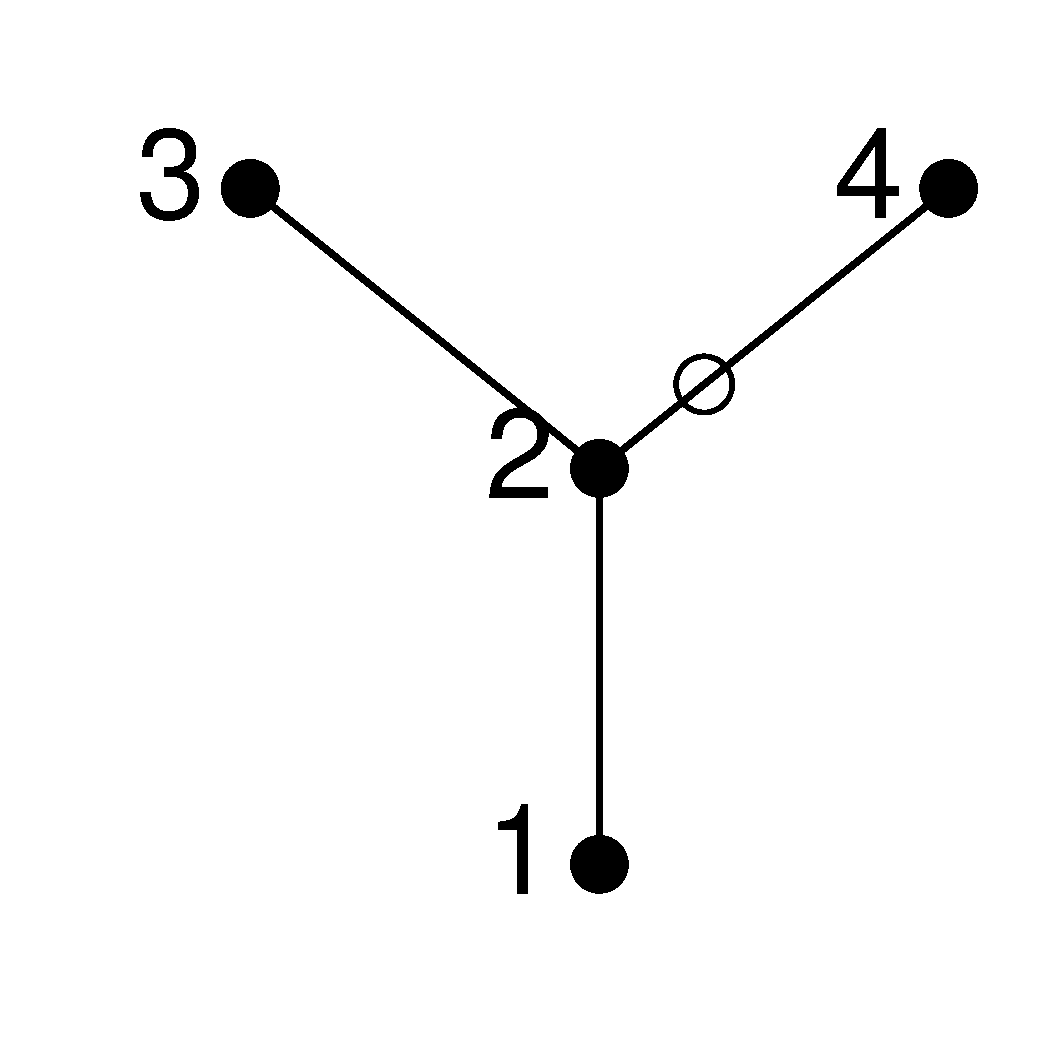
\includegraphics[width=.3\linewidth]{figure/Fig-App4LocNetwork-1.pdf}
	  \end{center}
	  \caption{A simple 4-location network, where each location is given by a solid circle numbered from 1 to 4, along with a prediction location, shown by the open circle. \label{fig:App4LocNet}}
  \end{figure}
\noindent
Let the linear distance between each connected location be 1 unit, so the distance matrix among the 4 locations, numbered sequentially for the rows and columns, is
\begin{singlespace}
\begin{knitrout}
\definecolor{shadecolor}{rgb}{0.969, 0.969, 0.969}\color{fgcolor}\begin{kframe}
\begin{alltt}
\hlstd{linDmat} \hlkwb{=} \hlkwd{rbind}\hlstd{(}
  \hlkwd{c}\hlstd{(}\hlnum{0}\hlstd{,}\hlnum{1}\hlstd{,}\hlnum{2}\hlstd{,}\hlnum{2}\hlstd{),}
  \hlkwd{c}\hlstd{(}\hlnum{1}\hlstd{,}\hlnum{0}\hlstd{,}\hlnum{1}\hlstd{,}\hlnum{1}\hlstd{),}
  \hlkwd{c}\hlstd{(}\hlnum{2}\hlstd{,}\hlnum{1}\hlstd{,}\hlnum{0}\hlstd{,}\hlnum{2}\hlstd{),}
  \hlkwd{c}\hlstd{(}\hlnum{2}\hlstd{,}\hlnum{1}\hlstd{,}\hlnum{2}\hlstd{,}\hlnum{0}\hlstd{))}
\end{alltt}
\end{kframe}
\end{knitrout}
\[
\bD = \left(
\begin{array}{cccc}
% latex table generated in R 3.4.3 by xtable 1.8-2 package
% Thu Jan 11 16:12:24 2018
 0 & 1 & 2 & 2 \\ 
  1 & 0 & 1 & 1 \\ 
  2 & 1 & 0 & 2 \\ 
  2 & 1 & 2 & 0 \\ 
  
\end{array}
\right)
\]
\end{singlespace}
\noindent I will use the Gaussian autocorrelation model, eqn 3, with $\sigma^2_p = 1$, $\alpha = 3$, and a small nugget effect, $\sigma_0 = 0.01$.  
\begin{knitrout}
\definecolor{shadecolor}{rgb}{0.969, 0.969, 0.969}\color{fgcolor}\begin{kframe}
\begin{alltt}
\hlstd{Sig} \hlkwb{=} \hlkwd{exp}\hlstd{(}\hlopt{-}\hlstd{(linDmat}\hlopt{/}\hlnum{3}\hlstd{)}\hlopt{^}\hlnum{2}\hlstd{)} \hlopt{+} \hlkwd{diag}\hlstd{(}\hlkwd{rep}\hlstd{(}\hlnum{0.01}\hlstd{,} \hlkwc{times} \hlstd{=} \hlnum{4}\hlstd{))}
\end{alltt}
\end{kframe}
\end{knitrout}
\begin{singlespace}
\begin{equation} \label{eq:appSigma}
\bSigma = \left(
\begin{array}{cccc}
% latex table generated in R 3.4.3 by xtable 1.8-2 package
% Thu Jan 11 16:12:24 2018
 1.010 & 0.895 & 0.641 & 0.641 \\ 
  0.895 & 1.010 & 0.895 & 0.895 \\ 
  0.641 & 0.895 & 1.010 & 0.641 \\ 
  0.641 & 0.895 & 0.641 & 1.010 \\ 
  
\end{array}
\right)
\end{equation}
\end{singlespace}
\noindent The spectral decomposition, $\bSigma = \bQ\bLambda\bQ\upp$ (eqn 10) is
\begin{singlespace}
\begin{knitrout}
\definecolor{shadecolor}{rgb}{0.969, 0.969, 0.969}\color{fgcolor}\begin{kframe}
\begin{alltt}
\hlstd{Lambda} \hlkwb{=} \hlkwd{diag}\hlstd{(}\hlkwd{eigen}\hlstd{(Sig)}\hlopt{$}\hlstd{values)}
\hlstd{Q} \hlkwb{=} \hlkwd{eigen}\hlstd{(Sig)}\hlopt{$}\hlstd{vectors}
\end{alltt}
\end{kframe}
\end{knitrout}
\begin{equation} \label{eq:appSpecDeco}
\bLambda= \left(
\begin{array}{cccc}
% latex table generated in R 3.4.3 by xtable 1.8-2 package
% Thu Jan 11 16:12:24 2018
 3.328 & 0.000 & 0.000 & 0.000 \\ 
  0.000 & 0.369 & 0.000 & 0.000 \\ 
  0.000 & 0.000 & 0.369 & 0.000 \\ 
  0.000 & 0.000 & 0.000 & -0.026 \\ 
  
\end{array}
\right)
\hspace{.3cm}
\bQ = \left(
\begin{array}{cccc}
% latex table generated in R 3.4.3 by xtable 1.8-2 package
% Thu Jan 11 16:12:24 2018
 -0.480 & 0.000 & 0.816 & -0.321 \\ 
  -0.556 & -0.000 & 0.000 & 0.831 \\ 
  -0.480 & -0.707 & -0.408 & -0.321 \\ 
  -0.480 & 0.707 & -0.408 & -0.321 \\ 
  
\end{array}
\right)
\end{equation}
\end{singlespace}
\noindent The eigenvectors, $\bv_i; i = 1,\ldots,4$, in $\bQ = [\bv_1|\bv_2|\bv_3|\bv_4]$ are orthonormal, which means that $\bv_i\upp \bv_j = 0$ if $i \ne j$, but $\bv_i\upp \bv_i = 1$.
\begin{singlespace}
\begin{knitrout}
\definecolor{shadecolor}{rgb}{0.969, 0.969, 0.969}\color{fgcolor}\begin{kframe}
\begin{alltt}
\hlkwd{t}\hlstd{(Q[,}\hlnum{1}\hlstd{])} \hlopt \hlstd{Q[,}\hlnum{4}\hlstd{]}
\end{alltt}
\begin{verbatim}
##              [,1]
## [1,] 2.775558e-17
\end{verbatim}
\begin{alltt}
\hlkwd{t}\hlstd{(Q[,}\hlnum{4}\hlstd{])} \hlopt \hlstd{Q[,}\hlnum{4}\hlstd{]}
\end{alltt}
\begin{verbatim}
##      [,1]
## [1,]    1
\end{verbatim}
\end{kframe}
\end{knitrout}
\end{singlespace}

Now, consider 4 random variables, $\bm Y = \{Y_1,Y_2,Y_3,Y_4\}$. The linear combination $\bv_4\upp\bm Y = -0.321Y_1 + 0.831Y_2 - 0.321Y_3 - 0.321Y_4$ is a perfectly valid construction, and must have a positive variance.  However, if $\bm Y$ has covariance matrix $\bSigma$ in \ref{eq:appSigma}, then $\var(\bv_4\upp\bm Y) = \bv_4\upp\bSigma\bv_4 = -0.026$, which is the 4th eigenvalue,
\begin{singlespace}
\begin{knitrout}
\definecolor{shadecolor}{rgb}{0.969, 0.969, 0.969}\color{fgcolor}\begin{kframe}
\begin{alltt}
\hlstd{v4} \hlkwb{=} \hlstd{Q[,}\hlnum{4}\hlstd{]}
\hlkwd{t}\hlstd{(v4)} \hlopt \hlstd{Sig} \hlopt \hlstd{v4}
\end{alltt}
\begin{verbatim}
##             [,1]
## [1,] -0.02611639
\end{verbatim}
\end{kframe}
\end{knitrout}
\end{singlespace}
\noindent which is not a valid variance, so $\bSigma$ in \ref{eq:appSigma} is not a valid covariance matrix.

To show how this works for kriging, consider predicting the location shown with the open circle in Figure~\ref{fig:App4LocNet}, which is 3/10 of the way from location 2 to location 4.  Then the distance from the 4 locations with solid circles in Figure~\ref{fig:App4LocNet} to the prediction location is the vector $(1.3, 0.3, 1.3, 0.7)$, and the covariances between the prediction location and the 4 locations with solid circles in Figure~\ref{fig:App4LocNet} is 
\begin{singlespace}
\begin{knitrout}
\definecolor{shadecolor}{rgb}{0.969, 0.969, 0.969}\color{fgcolor}\begin{kframe}
\begin{alltt}
\hlstd{cvec} \hlkwb{=} \hlkwd{exp}\hlstd{(}\hlopt{-}\hlstd{(}\hlkwd{c}\hlstd{(}\hlnum{1.3}\hlstd{,} \hlnum{0.3}\hlstd{,} \hlnum{1.3}\hlstd{,} \hlnum{0.7}\hlstd{)}\hlopt{/}\hlnum{3}\hlstd{)}\hlopt{^}\hlnum{2}\hlstd{)}
\hlstd{cvec}
\end{alltt}
\begin{verbatim}
## [1] 0.8287989 0.9900498 0.8287989 0.9470111
\end{verbatim}
\end{kframe}
\end{knitrout}
\end{singlespace}
\noindent Using eqn 7, the prediction variance of the location with the open circle, using data from the locations with the solid black circles, would be computed as
\begin{singlespace}
\begin{knitrout}
\definecolor{shadecolor}{rgb}{0.969, 0.969, 0.969}\color{fgcolor}\begin{kframe}
\begin{alltt}
\hlstd{(}\hlnum{1} \hlopt{+} \hlnum{0.01}\hlstd{)} \hlopt{-} \hlkwd{t}\hlstd{(cvec)} \hlopt \hlkwd{solve}\hlstd{(Sig)} \hlopt \hlstd{cvec} \hlopt{+}
  \hlstd{(}\hlnum{1} \hlopt{-} \hlstd{(}\hlkwd{sum}\hlstd{(}\hlkwd{solve}\hlstd{(Sig)} \hlopt \hlstd{cvec))}\hlopt{^}\hlnum{2}\hlstd{)}\hlopt{/}\hlkwd{sum}\hlstd{(}\hlkwd{solve}\hlstd{(Sig))}
\end{alltt}
\begin{verbatim}
##            [,1]
## [1,] -0.0425027
\end{verbatim}
\end{kframe}
\end{knitrout}
\end{singlespace}
\noindent which is negative, so we see that the larger matrix, where $\bSigma$ is appended with covariances that include the prediction location, eqn 9, is not a valid covariance matrix. 


%%%%%%%%%%%%%%%%%%%%%%%%%%%%%%%%%%%%%%%%%%%%%%%%%%%%%%%%%%%%%%%%%%%%%%%%%%%%%%%%%%
%%%%%%%%%%%%%%%%%%%%%%%%%%%%%%%%%%%%%%%%%%%%%%%%%%%%%%%%%%%%%%%%%%%%%%%%%%%%%%%%%%
%%%%%%%%%%%            %%%%%%%    %%%%%%%%  %%%%%%%       %%%%%%%%%%%%%%%%%%%%%%%%
%%%%%%%%%%%  %%%%%%%%%%%%%%%%%  %  %%%%%%%  %%%%%%%  %%%%  %%%%%%%%%%%%%%%%%%%%%%%
%%%%%%%%%%%  %%%%%%%%%%%%%%%%%  %%  %%%%%%  %%%%%%%  %%%%%%  %%%%%%%%%%%%%%%%%%%%%
%%%%%%%%%%%  %%%%%%%%%%%%%%%%%  %%%  %%%%%  %%%%%%%  %%%%%%%   %%%%%%%%%%%%%%%%%%%
%%%%%%%%%%%            %%%%%%%  %%%%  %%%%  %%%%%%%  %%%%%%%%  %%%%%%%%%%%%%%%%%%%
%%%%%%%%%%%  %%%%%%%%%%%%%%%%%  %%%%%  %%%  %%%%%%%  %%%%%%%   %%%%%%%%%%%%%%%%%%%
%%%%%%%%%%%  %%%%%%%%%%%%%%%%%  %%%%%%  %%  %%%%%%%  %%%%%%  %%%%%%%%%%%%%%%%%%%%%
%%%%%%%%%%%  %%%%%%%%%%%%%%%%%  %%%%%%%  %  %%%%%%%  %%%%  %%%%%%%%%%%%%%%%%%%%%%%
%%%%%%%%%%%            %%%%%%%  %%%%%%%%    %%%%%%%       %%%%%%%%%%%%%%%%%%%%%%%%
%%%%%%%%%%%%%%%%%%%%%%%%%%%%%%%%%%%%%%%%%%%%%%%%%%%%%%%%%%%%%%%%%%%%%%%%%%%%%%%%%%
%%%%%%%%%%%%%%%%%%%%%%%%%%%%%%%%%%%%%%%%%%%%%%%%%%%%%%%%%%%%%%%%%%%%%%%%%%%%%%%%%%


\end{spacing}

\end{document}


